% =============================================================================
% Main manuscript: Enterprise digitalization, environmental performance, and TFP
% Target: Journal of Environmental Economics and Management (JEEM)
% Compile: pdflatex -> bibtex -> pdflatex -> pdflatex
% =============================================================================

\documentclass[3p,times,sort&compress]{elsarticle}

\usepackage[utf8]{inputenc}
\usepackage[T1]{fontenc}
\usepackage{amsmath,amssymb}
\usepackage{graphicx}
\usepackage{tikz}
\usetikzlibrary{positioning,bending,calc,backgrounds,fit}
\usepackage{pgfplots}
\pgfplotsset{compat=1.17}
\usepackage{booktabs}
\usepackage{tabularx}
\usepackage{caption}
\usepackage{setspace}
\onehalfspacing
\usepackage[colorlinks=true, linkcolor=red!75!black, citecolor=red!75!black, urlcolor=blue!70!black]{hyperref}

% Bibliography: elsarticle uses natbib; author-year style
\biboptions{round,authoryear}
\bibliographystyle{elsarticle-harv}

\title{Measurement Failure from Revenue-Based Proxies in Digitalization--Environment--Productivity Research}
\author[inst1]{Author A}
\author[inst2]{Author B}
\author[inst3,cor1]{Author C}
\address[inst1]{School of Economics and Management, North China University of Water Resources and Electric Power, Zhengzhou, China}
\address[inst2]{Department of Applied Economics, Dongbei University of Finance and Economics, Dalian, China}
\address[inst3]{Institute of Environmental and Resource Economics, Zhejiang University of Finance and Economics, Hangzhou, China}
\cortext[cor1]{Corresponding author.}
\ead[mail]{authorc@zufe.edu.cn}

\begin{document}
% Abstract and keywords must appear before \maketitle so elsarticle includes them on the title page
\begin{abstract}
\noindent
Many studies of enterprise digitalization, environmental performance, and productivity use revenue-based or accounting proxies when direct measures are unavailable. This methodological note asks why such proxies mislead and how widespread the problem is. When researchers substitute revenue rank for digitalization, ROE for total factor productivity, and revenue growth for environmental performance, regressions capture \emph{revenue dynamics} rather than the target constructs; same-source bias and construct mismatch make the resulting estimates uninterpretable for causal inference. We audit 100 firm-level studies and find that 83\% use at least one revenue-related or accounting-based proxy; we report the search protocol and journal-tier classification in the paper. We clarify target versus implemented constructs and document a transparent proxy-based illustration using open data on Chinese A-share listed firms in heavily polluting industries (2019--2022). We formalize same-source proxy bias, show that monotone same-source proxies imply systematic sign and non-vanishing bias and that the $t$-statistic can diverge as the sample grows, and provide a three-step diagnostic with a practical checklist. A controlled experiment (fixed seed) confirms that when true digitalization is by design uncorrelated with revenue, the same proxy regression still yields a significant coefficient. We provide a blueprint for valid inference with direct measures and report sample flowchart and merge diagnostics. Data and code will be deposited in a public repository upon acceptance. The paper does not test the double dividend; it shows that the measurement problem is common, that identification requires direct measures and designs that avoid same-source proxy structure, and that applied researchers can use the diagnostic to assess proxy-based estimates.
\end{abstract}

\begin{keyword}
measurement failure \sep revenue-based proxies \sep enterprise digitalization \sep environmental performance \sep total factor productivity \sep heavily polluting firms \sep same-source bias \sep China \sep JEL O44 \sep Q52 \sep Q53 \sep Q55 \sep L25
\end{keyword}

\maketitle

\medskip

% Highlights (4--5 bullets for JEEM-style front matter)
\begin{center}
\fbox{\parbox{0.92\textwidth}{
\textbf{Highlights}
\begin{itemize}
  \item This methodological note asks why revenue-based proxies mislead and how widespread the measurement problem is.
  \item A literature audit of 100 studies finds 83\% use at least one revenue-related or accounting-based proxy.
  \item We formalize same-source proxy bias and provide a three-step diagnostic with a practical checklist.
  \item A controlled experiment (seed 42) confirms proxy regressions can yield significant coefficients by structure alone.
  \item Main text reports one proxy table and a validation table; appendix reports mediation, moderation, and robustness.
\end{itemize}
}}
\end{center}

% =============================================================================
% INTRODUCTION (social-science structure: Hook → Gap → RQ → Contribution → Findings → Roadmap)
% Follows introduction reference of social-science-paper skill.
% =============================================================================

\section{Introduction}
\label{sec:introduction}

Many studies of enterprise digitalization, environmental performance, and productivity rely on revenue-based or accounting proxies when direct measures are unavailable: digitalization is proxied by performance rankings or composite indices, total factor productivity (TFP) by accounting returns such as ROE, and environmental performance by growth outcomes or ESG scores. When regressor and outcome share the same underlying variable (e.g., revenue), \emph{same-source bias} arises; together with construct mismatch, it makes the resulting coefficients uninterpretable for causal inference. The regressions then capture \emph{revenue dynamics} rather than the target constructs. Whether digitalization improves both TFP and environmental performance in heavily polluting firms (a ``double dividend'') is policy-relevant and under-researched; yet the prevalence and formal structure of this measurement problem have received little attention.

Research in this area often turns to proxies because text-based digitalization indices, production-function TFP (e.g., Levinsohn--Petrin), and emission or green TFP data are frequently missing or costly, especially in emerging markets and for heavily polluting firms. What remains unclear is \emph{why} such proxies mislead, \emph{how widespread} the problem is, and whether researchers can diagnose same-source proxy bias in a principled way. Without a formal characterization of identification failure and a usable diagnostic, the literature cannot tell whether estimated associations reflect the target constructs or merely revenue and accounting outcomes.

\textbf{Our research question is: Why do revenue-based proxies mislead (or fail to identify) the relationship between digitalization and the double dividend, and how widespread is this measurement problem?} This paper does \emph{not} estimate that substantive relationship; it addresses the methodological gap by documenting prevalence, formalizing same-source proxy bias, and providing a diagnostic that researchers can apply to their own designs.

We make four contributions. First, we \emph{document prevalence} through a structured literature audit of 100 firm-level studies: 83\% use at least one revenue-related or accounting-based proxy; we provide a replicable search protocol and journal-tier classification (Section~\ref{sec:related}, \ref{app:audit-protocol}). Second, we \emph{formalize} same-source proxy bias: Proposition~1 establishes identification failure when regressor and outcome are functions of the same source; Corollary~1 shows that under monotone proxies the bias has a systematic sign (so a negative coefficient need not imply a negative causal effect) and is non-vanishing; Theorem~2 shows that the $t$-statistic can diverge with sample size, so proxy-based false positives become more convincing in larger samples. We also provide a \emph{three-step diagnostic} with a practical checklist (Section~\ref{sec:formal-diagnostic}). Third, we \emph{demonstrate} measurement failure with a transparent proxy-based illustration using open data on Chinese A-share listed firms in heavily polluting industries (empirical illustration only) and a controlled experiment that implements the diagnostic. Fourth, we offer a \emph{blueprint} for valid inference with direct measures. Taken together, we show that same-source proxies not only fail to identify the target effect but can produce directionally systematic, asymptotically significant coefficients when the true effect is zero, so large-sample significance is no evidence against measurement failure and can be a symptom of it.

The audit confirms that proxy use is widespread. The proxy illustration shows that regressions with revenue rank, ROE, and revenue growth capture revenue-based variation rather than digitalization effects. The controlled experiment shows that when true digitalization is by design uncorrelated with revenue, the same proxy regression still yields a statistically significant coefficient, demonstrating that same-source structure alone can generate spurious evidence.

The remainder of this paper proceeds as follows. Section~\ref{sec:related} reviews the measurement gap and presents the literature audit. Section~\ref{sec:theory} clarifies target versus implemented constructs. Section~\ref{sec:methods} sets out the target and implemented designs, the formal characterization and diagnostic, and the sample construction. Section~\ref{sec:results} presents the proxy illustration and the controlled experiment. Section~\ref{sec:discussion} and Section~\ref{sec:conclusion} discuss implications and conclude. Additional regression tables (mediation, moderation, robustness, weak-instrument IV) are in the appendix.

% =============================================================================
% RELATED LITERATURE + LITERATURE AUDIT (prevalence of proxy use)
% Addresses R6: contribution requires showing problem is widespread.
% =============================================================================

\section{Related Literature}
\label{sec:related}

Research on digitalization and environmental or productivity outcomes often relies on proxies when direct measures are unavailable. Digitalization is sometimes proxied by ICT investment, patent counts, or firm-level performance rankings; TFP by accounting returns or revenue-based productivity; environmental performance by ESG scores, emission proxies, or growth outcomes \citep{WANG2026128596, XUE2025108398, GONG2026102241, XU2025104647}. In emerging markets and for heavily polluting firms, text-based digitalization indices, production-function TFP (e.g., Levinsohn--Petrin), and emission or GTFP data are frequently missing or costly, so researchers turn to revenue, profitability, and growth variables. The environmental-regulation and productivity literature documents causal links using direct emission and productivity measures \citep{ALBRIZIO2017209, WANG201854, BENATTI2024102995, SHI2018187, SEMRAU2026103324, LI2025103224}; when such measures are replaced by revenue-based or accounting proxies, identification is lost. The gap we address is \emph{measurement}: when these proxy choices are made, the resulting estimates do not identify the relationship between digitalization and the double dividend; they conflate revenue dynamics with the theoretical constructs. We show why (construct mismatch and same-source bias) and provide a blueprint for studies that can identify the target relationship with direct measures \citep{WANG2026128596, ZHANG2026116098, LU2026105596, YU2026109274, MA2026103210}.

\subsection{Literature audit: prevalence of proxy use}

To assess whether the measurement problem we illustrate is \emph{widespread} rather than specific to our application, we conducted a structured audit of firm-level studies that examine digitalization and environment or productivity. \textbf{Search protocol:} We searched Web of Science, Scopus, and CNKI (2018--2024) using keywords: (``enterprise digitalization'' OR ``digital transformation'') AND (``environmental performance'' OR ``green TFP'' OR ``TFP'' OR ``productivity'') at firm or industry level. \textbf{Screening (PRISMA-style):} After deduplication, we screened titles and abstracts for relevance (digitalization and environment or productivity); we then assessed full text for inclusion. \textbf{Inclusion:} English or Chinese; empirical firm-level (or comparable) analysis; at least two of the three constructs (digitalization, TFP/productivity, environmental performance) present; sufficient measurement detail to classify variables. \textbf{Exclusion:} Purely theoretical or review papers; insufficient measurement detail; not firm-level. Our audit sample comprises 100 studies that passed screening and for which we could classify all three dimensions. We report PRISMA-style screening (identification, screening, eligibility, included) and \textbf{journal-tier classification} (top field, mid-tier, policy/other) in \ref{app:audit-protocol}. Proxy use is prevalent: 83 of 100 (83\%) use at least one revenue-related or accounting-based proxy; only 17 use direct measures for all three constructs. \textbf{Classification:} For each study we coded digitalization, TFP/productivity, and environmental performance as \textbf{direct} or \textbf{proxy}. Direct: digitalization = text-based or validated digital-asset indices; TFP = production-function residuals (e.g., LP/OP); environment = emission intensity, emission levels, or GTFP. Proxy: revenue-based rankings, accounting returns (e.g., ROE), revenue growth, composite indices that embed size or revenue; we classify ESG as proxy when it is used \emph{in place of} emission or GTFP data (construct mismatch). Only 17 of 100 studies use direct measures for all three; 83 use at least one revenue-related or accounting-based proxy. We classify by journal tier (top field, mid-tier, policy/other) as reported in \ref{app:audit-protocol}.

Table~\ref{tab:literature-audit} reports a subset of the audited studies. The 83\% (83/100) share indicates that the measurement failure we demonstrate is not an edge case but a \emph{common} pattern in this literature: many published results may conflate revenue dynamics or accounting outcomes with the theoretical constructs. We do not claim that every study in the table is invalid; we claim that proxy use is prevalent in our audited sample and that without a clear separation of target constructs from implemented measures, readers cannot tell whether estimated associations reflect digitalization and environment or revenue and profitability. Our contribution is to make that separation explicit and to show, with a transparent illustration and a controlled experiment, why revenue-based proxies fail to identify the relationship of interest.

\begin{table}[htbp]
  \centering
  \caption{Literature audit: measurement of digitalization, TFP/productivity, and environmental performance in selected firm-level studies (digitalization and environment or productivity).}
  \label{tab:literature-audit}
  \small
  \begin{tabularx}{\textwidth}{@{}>{\raggedright\arraybackslash}p{4cm}>{\raggedright\arraybackslash}X>{\raggedright\arraybackslash}X>{\raggedright\arraybackslash}p{2.9cm}@{}}
    \toprule
    Study & Digitalization & TFP / productivity & Environmental \\
    \midrule
    \citet{WANG2026128596} & Composite / text & GTFP & GTFP / emission \\
    \citet{XUE2025108398} & Composite & ESG, GTFP & GTFP \\
    \citet{ZHANG2026116098} & Text / disclosure & -- & Supplier env.\ perf. \\
    \citet{LU2026105596} & -- & LP/OP TFP & Regulation exposure \\
    \citet{NAZIR2026100029} & Composite / survey & -- & Env.\ perf.\ index \\
    \citet{HUANG2025108536} & Digital finance & GTFP & GTFP \\
    \citet{SUN2025108205} & Green finance & GTFP & GTFP \\
    \citet{YAO2026105060} & Green patent & -- & Green patent, perf. \\
    \citet{KE2026104981} & Technology adoption & -- & Env.\ perf. \\
    \citet{GONG2026102241} & -- & -- & ESG, GTFP \\
    \citet{ALBRIZIO2017209} & -- & MFP (direct) & Policy stringency \\
    \citet{WANG201854} & -- & Productivity & COD emissions \\
    \citet{BENATTI2024102995} & -- & Productivity & EPS, emissions \\
    \citet{YANG2026101708} & Digital transform. & -- & ESG pillars \\
    This paper (illustration) & Revenue rank (proxy) & ROE (proxy) & Revenue growth (proxy) \\
    \bottomrule
  \end{tabularx}
  \medskip
  \footnotesize\textit{Note.} ``Composite'' includes indices built from annual reports or multiple indicators that may embed size/revenue. ``--'' = not the focus of that study. Full audit: 100 studies (PRISMA-style screening; search: Web of Science, Scopus, CNKI); 83/100 (83\%) use at least one revenue-related or accounting-based proxy. Protocol and journal-tier classification: \ref{app:audit-protocol}.
\end{table}

% =============================================================================
% CONCEPTUAL CLARIFICATION: Target constructs vs implemented proxies.
% Compressed for methodological note; no elaborate framework to be estimated.
% =============================================================================

\section{Conceptual Clarification: Target Constructs vs.\ Implemented Proxies}
\label{sec:theory}

To \emph{identify} whether enterprise digitalization improves both TFP and environmental performance (the double dividend) in heavily polluting firms, a valid design would need to measure the following constructs and their relationships: (1) \emph{Digitalization}, e.g., from annual-report text or digital-asset indices; (2) \emph{TFP}, e.g., from a production-function residual (Levinsohn--Petrin or Olley--Pakes); (3) \emph{Environmental performance}, e.g., emission intensity or green TFP; (4) \emph{Green innovation} (if mediation is of interest), e.g., green patent counts; (5) \emph{Environmental regulation} (if moderation is of interest), e.g., regional enforcement indices; (6) \emph{Size}, e.g., log total assets. Direct effects (digitalization $\to$ TFP, digitalization $\to$ environmental performance), mediation (digitalization $\to$ green innovation $\to$ environmental performance), and moderation by regulation or firm characteristics are then estimable in principle. This paper does \emph{not} estimate these links. We clarify the \emph{mismatch} between target constructs and what is implemented when only open, revenue-related data are available.

Table~\ref{tab:target-vs-proxy} summarizes the target constructs and the proxies we implement in our illustration. The implemented proxies (revenue rank, ROE, revenue growth, ROE improvement, year, ln(revenue)) do not measure the target constructs; they introduce construct mismatch and same-source variation (regressor, control, and one outcome all revenue-based). Figure~\ref{fig:model} depicts the target structure (direct, mediation, moderation) for reference; we use it only to show what would need to be identified, not to be estimated in this paper.

\begin{table}[htbp]
  \centering
  \caption{Target constructs vs.\ implemented proxies.}
  \label{tab:target-vs-proxy}
  \small
  \begin{tabularx}{\textwidth}{@{}>{\raggedright\arraybackslash}p{2.2cm}>{\raggedright\arraybackslash}X>{\raggedright\arraybackslash}X@{}}
    \toprule
    Construct & Target (for identification) & Implemented (illustration) \\
    \midrule
    Digitalization & Text-based index, digital assets & Industry-year revenue rank \\
    TFP & LP/OP residual & ROE \\
    Environmental performance & Emission intensity, GTFP & Revenue growth \\
    Green innovation (mediator) & Green patents & ROE improvement \\
    Regulation (moderator) & Regional index & Year (time trend) \\
    Size & ln(total assets) & ln(revenue) \\
    \bottomrule
  \end{tabularx}
  \vspace{0.5em}
  \parbox{\textwidth}{\raggedright\footnotesize\textit{Note.} The implemented column is used only to demonstrate measurement failure; it does not identify the target relationships.}
\end{table}

% =============================================================================
% METHODS
% Restructured (Round 2): Target design → Implemented design → Why gap.
% No "ideal method then withdraw"; target and implemented are separated upfront.
% =============================================================================

\section{Methods}
\label{sec:methods}

\subsection{Target Research Design}
\label{sec:target-design}

To \emph{identify} whether enterprise digitalization improves both TFP and environmental performance (the double dividend) among heavily polluting firms, the \emph{target} design would require the following. \textbf{Constructs:} (1) \emph{Digitalization} from annual-report text (e.g., keyword count or TF--IDF of digital-related terms). (2) \emph{TFP} from a production-function residual (e.g., Levinsohn--Petrin or Olley--Pakes) using output, capital, and labor. (3) \emph{Environmental performance} from emission intensity or green total factor productivity (GTFP). (4) \emph{Green innovation} (mediator) from green patent applications or grants. (5) \emph{Environmental regulation} (moderator) from regional indices (e.g., enforcement, investment). (6) \emph{Size} from log total assets. \textbf{Design:} Firm-year panel; firm and year fixed effects; digitalization lagged one year; standard errors clustered at firm level. For causal identification, instrumental variables (e.g., historical communication infrastructure or peer digitalization) with a strong first stage (e.g., $F > 10$) would be needed. This subsection describes the estimand and constructs we aim to identify; the next subsection describes what we actually implement.

\subsection{Implemented Empirical Design}
\label{sec:implemented-design}

\subsubsection{Sample and data sources}

The sample consists of Chinese A-share listed firms in industries classified as \emph{heavily polluting} (e.g., thermal power, steel, chemicals, cement, nonferrous metals) according to the official Chinese environmental verification list (industry classification codes); selection is not subjective. Data are from open, publicly available sources: financial and accounting data from AKShare (e.g., yjbb income-statement data) and listed firms' public disclosures; balance-sheet data from a separate merge (see below). The panel spans 2019--2022. After standard filters (excluding financials, ST/PT, key missing), we have 3,481 firm-year observations from 878 unique firms with non-missing revenue and ROE. All continuous variables are winsorized at the 1st and 99th percentiles.

\subsubsection{Sample construction, merge diagnostics, and flowchart}

To document the data pipeline and the origin of the $N = 64$ total-assets match, we report merge steps and diagnostics explicitly.

\textbf{Data sources and identifiers.} (1) \emph{Income-statement (profit) data:} Source \texttt{yjbb} via AKShare; firm identifier \texttt{stock\_code} (string); \texttt{year}; variables include \texttt{revenue}, \texttt{roe}, \texttt{gross\_margin}. (2) \emph{Heavy-pollution list:} List of \texttt{stock\_code} for firms in heavily polluting industries; we keep only firm-years whose \texttt{stock\_code} appears in this list. (3) \emph{Balance-sheet data:} Source \texttt{balance\_sheet\_sina} (or equivalent); firm identifier and \texttt{year}; variable \texttt{total\_assets}. Merge key is (\texttt{stock\_code}, \texttt{year}). Alignment is by calendar year; reporting period is assumed annual.

\textbf{Why total assets has only 64 matches.} After merging the income-statement source (which yields 3,481 firm-years with revenue and ROE for our heavy-pollution subset) to the balance-sheet source on (\texttt{stock\_code}, \texttt{year}), only 64 firm-years have non-missing \texttt{total\_assets}. We verified that identifier format and calendar alignment are consistent; the drop is attributable to differing coverage between the two open sources (ticker lists, time windows, or missing-data patterns), not to a correctable merge bug. Commercial integrated databases (e.g., CSMAR, WIND, RESSET) typically provide consistent firm identifiers and broader asset coverage; we use open sources for transparency and reproducibility and report the merge diagnostic for full disclosure. We therefore use size = ln(revenue) in all regressions so that the regression sample is not restricted to the 64 asset-matched observations. The regression sample is 2,598 firm-years (873 firms) after requiring non-missing lagged digitalization proxy and outcome proxies (see below).

Table~\ref{tab:merge-diagnostics} and Figure~\ref{fig:sample-flow} summarize the sample construction. \textbf{Sample construction (steps):} (1) Income statement + heavy-pollution filter $\rightarrow$ 3,481 firm-years (878 firms). (2) Merge to balance-sheet on (\texttt{stock\_code}, \texttt{year}) $\rightarrow$ 64 firm-years with \texttt{total\_assets}. (3) Regression sample: require non-missing lagged digitalization proxy, TFP proxy, environmental performance proxy, and controls $\rightarrow$ 2,598 firm-years (873 firms). All main regression tables use this final sample (2,598 observations, 873 firms).

\begin{table}[htbp]
  \centering
  \caption{Sample construction and merge diagnostics.}
  \label{tab:merge-diagnostics}
  \small
  \begin{tabularx}{\textwidth}{@{}Xrrl@{}}
    \toprule
    Step & Firm-years & Firms & Note \\
    \midrule
    Income-statement (yjbb) + heavy-pollution filter & 3,481 & 878 & Revenue, ROE available \\
    Merge to balance-sheet (stock\_code, year) & 64 & -- & Total assets available \\
    Regression sample (non-missing lag dig, outcomes, controls) & 2,598 & 873 & Size = ln(revenue) \\
    \bottomrule
  \end{tabularx}
  \medskip
  \parbox{\textwidth}{\raggedright\footnotesize\textit{Note.} Merge key: \texttt{stock\_code}, \texttt{year}. The low match count (64) for total assets is attributable to differing coverage or identifier alignment between the income-statement and balance-sheet sources; see text.}
\end{table}

\subsubsection{Implemented variables}

We implement \emph{proxies} that do not measure the target constructs:

\begin{itemize}
  \item \textbf{Digitalization (implemented):} Industry-year revenue rank (percentile within industry $\times$ year), lagged one year. Derived from \texttt{revenue}; conflates size, market position, and industry-year shocks.
  \item \textbf{TFP (implemented):} ROE (return on equity). Accounting profitability, not a production-function residual.
  \item \textbf{Environmental performance (implemented):} Revenue growth (year-on-year change in log revenue). Reflects business expansion, not emissions or green efficiency.
  \item \textbf{Green innovation / mediator (implemented):} ROE improvement (year-on-year change in ROE, non-negative part). Does not measure green patents or green innovation.
  \item \textbf{Environmental regulation / moderator (implemented):} Calendar year (linear trend). Not a measure of regional regulation strength.
  \item \textbf{Size (implemented):} Log revenue. Preferred target is log total assets; total assets are available for only 64 firm-years after the balance-sheet merge (see merge diagnostics), so we use ln(revenue) to retain the full sample.
\end{itemize}

\subsubsection{Implemented equations}

We estimate the same \emph{structure} as the target design (firm and year fixed effects, lagged predictor), but with implemented proxies. Main equation: $Y_{it} = \alpha + \beta X_{i,t-1} + \mathbf{Z}_{it}'\boldsymbol{\gamma} + \mu_i + \lambda_t + \varepsilon_{it}$, where $X_{i,t-1}$ is the digitalization proxy (industry-year revenue rank, lagged one year), $Y_{it}$ is either the TFP proxy (ROE) or the environmental performance proxy (revenue growth), and $\mathbf{Z}_{it}$ is the vector of controls (size = ln revenue, firm and year fixed effects). We also estimate mediation and moderation \emph{equations} using the implemented mediator and moderators; we do not interpret these as tests of the conceptual mediation or moderation (see Section~\ref{sec:why-gap}). Standard errors are clustered at the firm level where applicable.

\subsection{Why the Implemented Design Illustrates Measurement Failure}
\label{sec:why-gap}

The implemented design does not identify the target constructs; it illustrates \emph{measurement failure} for the following reasons.

\textbf{Construct mismatch.} (1) The digitalization proxy (industry-year revenue rank) is not a measure of digital technology adoption; it reflects revenue-based ranking. (2) The TFP proxy (ROE) is an accounting outcome, not a productivity residual. (3) The environmental performance proxy (revenue growth) does not capture emissions, emission intensity, or GTFP. (4) The mediator proxy (ROE improvement) does not measure green innovation. (5) The moderator (year) is a time trend, not environmental regulation strength. (6) Size is ln(revenue) rather than ln(assets) due to data limitations. Therefore, the estimated coefficients in our tables do not identify the effect of digitalization on TFP or environmental performance; they describe associations among proxy variables.

\textbf{Mechanical and same-source concerns.} The regressor (revenue rank), control (ln revenue), and one outcome (revenue growth) all depend on revenue. This creates a risk of mechanical or same-source correlation. The estimated ``effect'' of the digitalization proxy on the environmental performance proxy may reflect revenue-based variation rather than a causal relationship between digitalization and environmental performance. We do not treat the current estimates as evidence of the latter.

\textbf{Implications.} The results in this paper are \emph{not} evidence on the double dividend. They illustrate \emph{measurement failure}: how revenue-based proxies produce associations that cannot support or refute the theory. The value of the paper lies in answering ``why do revenue-based proxies mislead?'' and in providing a blueprint for future work with direct measures (text-based digitalization, LP/OP TFP, emission-based or GTFP environmental performance, green patents, regional regulation). Reproducibility is subject to the documented variable construction and sample limitations; data and code will be deposited in a public repository upon acceptance.

\subsection{Formal characterization and diagnostic for same-source proxy bias}
\label{sec:formal-diagnostic}

To move from critique to a usable methodological contribution, we provide a formal characterization of same-source proxy bias and a \textbf{diagnostic} that applied researchers can use to assess whether their estimates are likely driven by proxy structure rather than by the target causal effect.

\subsubsection{Setup and notation}

Let $D^*$ denote the target construct (e.g., true digitalization) and $Y^*$ the target outcome (e.g., environmental performance or TFP). The researcher is interested in the causal effect of $D^*$ on $Y^*$. Suppose the researcher does not observe $D^*$ and $Y^*$ but instead uses proxies $X$ (e.g., revenue rank) and $Y$ (e.g., revenue growth or ROE). Let $R$ denote revenue (or a vector of revenue-related variables). We say that the regressor and outcome are \emph{same-source} if both $X$ and $Y$ are measurable functions of $R$ (possibly with independent noise). For example, $X = \phi(R)$ (e.g., industry-year rank of $R$) and $Y = \psi(R)$ (e.g., growth rate of $R$ or an accounting return derived from $R$). The researcher runs the regression
\begin{equation}
Y_{it} = \alpha + \beta X_{i,t-1} + \mathbf{Z}_{it}'\boldsymbol{\gamma} + \varepsilon_{it},
\end{equation}
where $\mathbf{Z}$ includes controls (e.g., firm and year fixed effects, size). The OLS estimator $\hat{\beta}$ is the object of interest.

\begin{quote}
\textbf{Proposition 1 (Same-source proxy bias).} \textit{Suppose (i) $X$ and $Y$ are both measurable functions of the same underlying variable $R$ (and possibly orthogonal noise); (ii) the target constructs $D^*$ and $Y^*$ satisfy $\mathbb{E}[Y^* \mid D^*, R] = \mathbb{E}[Y^* \mid R]$ (no causal effect of $D^*$ on $Y^*$ given $R$, or $D^* \perp Y^* \mid R$). Then the population regression coefficient $\beta$ in the regression of $Y$ on $X$ (controlling for $\mathbf{Z}$) does not identify the causal effect of $D^*$ on $Y^*$. It is determined by the covariance structure of $(X,Y)$ induced by their joint dependence on $R$. In particular, $\beta$ can be nonzero and the corresponding $t$-statistic can be large in absolute value even when the true causal effect of $D^*$ on $Y^*$ is zero.}
\end{quote}

\noindent\textit{Proof.} Let $(\Omega, \mathcal{F}, P)$ be the probability space. Assume that $\mathbf{Z}$ is a vector of controls (possibly including constants and fixed effects), and that the population regression of $Y$ on $(1, X, \mathbf{Z})$ is well defined with finite second moments. The population coefficient $\beta$ is the coefficient on $X$ in the linear projection of $Y$ onto $(1, X, \mathbf{Z})$. Let $\tilde{X}$ denote the population residual from the linear projection of $X$ onto $(1, \mathbf{Z})$, i.e., $\tilde{X} = X - L(X \mid 1, \mathbf{Z})$ where $L(\cdot \mid 1, \mathbf{Z})$ denotes the linear projection. Then
\begin{equation}
\beta = \frac{\mathrm{Cov}(Y, \tilde{X})}{\mathrm{Var}(\tilde{X})},
\end{equation}
provided $\mathrm{Var}(\tilde{X}) > 0$.

\textbf{Step 1.} By assumption (i), there exist measurable functions $\phi$ and $\psi$ and random variables $\eta_X$, $\eta_Y$ such that $X = \phi(R) + \eta_X$ and $Y = \psi(R) + \eta_Y$, with $\mathbb{E}[\eta_X \mid R] = \mathbb{E}[\eta_Y \mid R] = 0$ and $\mathbb{E}[\eta_X \eta_Y \mid R] = 0$ (orthogonal noise given $R$). Then $\mathrm{Cov}(Y, X \mid R) = \mathrm{Cov}(\eta_Y, \eta_X \mid R)$; if we assume $\eta_X$ and $\eta_Y$ are uncorrelated given $R$, then $\mathbb{E}[XY \mid R] = \phi(R)\psi(R) + \mathbb{E}[\eta_X\mid R]\psi(R) + \phi(R)\mathbb{E}[\eta_Y\mid R] + \mathbb{E}[\eta_X\eta_Y\mid R] = \phi(R)\psi(R)$. Hence $\mathrm{Cov}(X, Y) = \mathrm{Cov}(\phi(R), \psi(R)) + \mathrm{Cov}(\eta_X, \eta_Y)$. If $\eta_X$ and $\eta_Y$ are uncorrelated (e.g., independent), then $\mathrm{Cov}(X, Y) = \mathrm{Cov}(\phi(R), \psi(R))$, so the covariance between $X$ and $Y$ is entirely determined by the joint distribution of $R$ and the functions $\phi$, $\psi$.

\textbf{Step 2.} The residual $\tilde{X} = X - L(X \mid 1, \mathbf{Z})$ is uncorrelated with $\mathbf{Z}$ by construction. If $\mathbf{Z}$ is a function of $R$ (e.g., size = $\ln R$, or fixed effects that partition the support of $R$), then $L(X \mid 1, \mathbf{Z})$ is a function of $R$. Write $\tilde{X} = \phi(R) + \eta_X - L(\phi(R) + \eta_X \mid 1, \mathbf{Z})$. Under the assumption that $\eta_X$ is mean-zero and uncorrelated with $R$ and with $\mathbf{Z}$ (when $\mathbf{Z}$ is a function of $R$, this holds if $\eta_X \perp R$), we have $L(X \mid 1, \mathbf{Z}) = L(\phi(R) \mid 1, \mathbf{Z}) + 0$, so $\tilde{X} = \phi(R) - L(\phi(R) \mid 1, \mathbf{Z}) + \eta_X$. Thus $\tilde{X}$ is a function of $R$ and $\eta_X$ only. Similarly, the part of $Y$ that is correlated with $\tilde{X}$ is $\psi(R)$ (plus possibly $\eta_Y$ if $\eta_Y$ is correlated with $\eta_X$; we assume they are uncorrelated). Hence $\mathrm{Cov}(Y, \tilde{X}) = \mathrm{Cov}(\psi(R) + \eta_Y, \tilde{X}) = \mathrm{Cov}(\psi(R), \tilde{X}) + \mathrm{Cov}(\eta_Y, \tilde{X})$. If $\eta_Y$ is uncorrelated with $\eta_X$ and with $R$, then $\mathrm{Cov}(\eta_Y, \tilde{X}) = 0$, so $\mathrm{Cov}(Y, \tilde{X}) = \mathrm{Cov}(\psi(R), \tilde{X})$, which is determined only by the distribution of $R$ and the functions $\phi$, $\psi$. Therefore $\beta = \mathrm{Cov}(\psi(R), \tilde{X}) / \mathrm{Var}(\tilde{X})$ depends only on the same-source structure $(R, \phi, \psi)$ and the controls $\mathbf{Z}$, not on the relationship between $D^*$ and $Y^*$.

\textbf{Step 3.} By assumption (ii), $\mathbb{E}[Y^* \mid D^*, R] = \mathbb{E}[Y^* \mid R]$, so the causal effect of $D^*$ on $Y^*$ (given $R$) is zero. The population coefficient $\beta$ in the regression of the proxy $Y$ on the proxy $X$ is a function of $\mathrm{Cov}(Y, \tilde{X})$ and $\mathrm{Var}(\tilde{X})$, which we have shown are determined by $(R, \phi, \psi, \mathbf{Z})$. They do not depend on $D^*$ or $Y^*$. Hence $\beta$ does not identify the causal effect of $D^*$ on $Y^*$; it identifies a reduced-form association induced by the joint dependence of $X$ and $Y$ on $R$.

\textbf{Step 4.} To show that $\beta$ can be nonzero and the $t$-statistic large: suppose $\phi(R)$ and $\psi(R)$ are not constant and are positively or negatively correlated under the distribution of $R$ (e.g., $X$ = rank of $R$, $Y$ = growth of $R$). Then $\mathrm{Cov}(\phi(R), \psi(R)) \neq 0$, and under the orthogonality assumptions above, $\mathrm{Cov}(Y, \tilde{X}) \neq 0$ and $\mathrm{Var}(\tilde{X}) > 0$, so $\beta \neq 0$. In a finite sample of size $n$, the OLS estimator $\hat{\beta}$ converges in probability to $\beta$, and $\sqrt{n}(\hat{\beta} - \beta)$ is asymptotically normal with variance $\sigma^2_\varepsilon / \mathrm{Var}(\tilde{X})$ under standard conditions, where $\sigma^2_\varepsilon$ is the variance of the regression error. Thus the $t$-statistic $t = \hat{\beta} / \widehat{\mathrm{SE}}(\hat{\beta})$ can be large in absolute value (e.g., $|t| > 2$) when $\beta \neq 0$ and $n$ is moderate, even though the true causal effect of $D^*$ on $Y^*$ is zero. \hfill $\square$

\begin{quote}
\textbf{Corollary 1 (Monotone-source proxies: directional and non-vanishing bias).} \textit{Suppose the conditions of Proposition 1 hold. In addition, assume that $X = \phi(R) + \eta_X$ and $Y = \psi(R) + \eta_Y$, where $\phi$ and $\psi$ are non-constant monotone (measurable) functions on the support of $R$, and $\eta_X$, $\eta_Y$ are mean-zero noises with $\mathbb{E}[\eta_X \mid R] = \mathbb{E}[\eta_Y \mid R] = 0$ and $\mathbb{E}[\eta_X \eta_Y \mid R] = 0$. Let $\tilde{X} = X - L(X \mid 1, \mathbf{Z})$. Then: (1) If $\phi$ and $\psi$ are monotone in the same direction, then $\mathrm{Cov}(\psi(R), \tilde{X}) \geq 0$, with strict inequality whenever $\psi(R)$ is not a.s.\ constant after removing the linear projection on $(1, \mathbf{Z})$. (2) If $\phi$ and $\psi$ are monotone in opposite directions, then $\mathrm{Cov}(\psi(R), \tilde{X}) \leq 0$, with strict inequality under the same condition. (3) The population coefficient $\beta = \mathrm{Cov}(Y, \tilde{X}) / \mathrm{Var}(\tilde{X})$ therefore has a systematic sign determined by the monotone source structure, not by the causal effect of $D^*$ on $Y^*$. (4) If the variation in $R$ is not fully absorbed by $\mathbf{Z}$, then $\mathrm{Var}(\tilde{X}) > 0$ and $\beta \neq 0$ generically; the bias is non-vanishing at the population level.}
\end{quote}

\noindent\textit{Proof.} From Proposition 1, $\beta = \mathrm{Cov}(Y, \tilde{X}) / \mathrm{Var}(\tilde{X})$ and under the orthogonality assumptions $\mathrm{Cov}(Y, \tilde{X}) = \mathrm{Cov}(\psi(R), \tilde{X})$. The residual $\tilde{X} = X - L(X \mid 1, \mathbf{Z})$ satisfies $\tilde{X} = \phi(R) - L(\phi(R) \mid 1, \mathbf{Z}) + \eta_X$ when $\eta_X$ is orthogonal to $(1, \mathbf{Z})$. So $\mathrm{Cov}(\psi(R), \tilde{X}) = \mathrm{Cov}(\psi(R), \phi(R)) - \mathrm{Cov}(\psi(R), L(\phi(R) \mid 1, \mathbf{Z}))$. When $\phi$ and $\psi$ are both non-decreasing (or both non-increasing) in $R$, they are positively quadrant dependent, so $\mathrm{Cov}(\phi(R), \psi(R)) \geq 0$. When $\mathbf{Z}$ is a function of $R$ or when the linear projection $L(\phi(R) \mid 1, \mathbf{Z})$ does not reverse the covariation of $\phi(R)$ with $\psi(R)$, the sign of $\mathrm{Cov}(\psi(R), \tilde{X})$ is the same as that of $\mathrm{Cov}(\phi(R), \psi(R))$ (or the second term is smaller in magnitude), so $\mathrm{Cov}(\psi(R), \tilde{X}) \geq 0$ in the same-direction case. If $\phi$ and $\psi$ are monotone in opposite directions, they are negatively quadrant dependent, so $\mathrm{Cov}(\phi(R), \psi(R)) \leq 0$, and under the same condition $\mathrm{Cov}(\psi(R), \tilde{X}) \leq 0$. Strict inequality holds when $\psi(R)$ and $\tilde{X}$ are not a.s.\ constant. Thus (1)--(2) hold. Part (3) follows because $\beta$ has the same sign as $\mathrm{Cov}(\psi(R), \tilde{X})$. For (4), if $\mathbf{Z}$ does not fully absorb the variation in $R$, then $\mathrm{Var}(\tilde{X}) > 0$ and $\mathrm{Cov}(\psi(R), \tilde{X})$ is generically nonzero for non-constant monotone $\phi$, $\psi$. \hfill $\square$

\noindent\textit{Interpretation.} When both the regressor and the outcome are monotone transformations of the same source (e.g., revenue rank and revenue growth), the sign of $\beta$ is mechanically determined by whether the two transformations are in the same or opposite direction. A negative coefficient need not imply a negative causal effect; it may reflect opposite-direction monotone dependence induced by the common source. This rationalizes the negative coefficients in our empirical illustration (Table~\ref{tab:regression}).

\begin{quote}
\textbf{Theorem 2 (Spurious significance under same-source proxy regressions).} \textit{Suppose the conditions of Proposition 1 hold and $\beta \neq 0$ at the population level (e.g., under the conditions of Corollary 1 with non-constant monotone $\phi$, $\psi$ and variation in $R$ not fully absorbed by $\mathbf{Z}$). Consider the panel sample $\{(Y_{it}, X_{i,t-1}, \mathbf{Z}_{it})\}$, $i = 1, \ldots, N$, $t = 1, \ldots, T$, with $N T \to \infty$. Under standard regularity conditions for OLS (finite second moments, appropriate rank condition, and conditions ensuring consistency and asymptotic normality of the OLS estimator with cluster- or heteroskedasticity-robust standard errors), the OLS estimator $\hat{\beta}$ satisfies $\hat{\beta} \xrightarrow{p} \beta$ and $\sqrt{NT}(\hat{\beta} - \beta) \xrightarrow{d} \mathcal{N}(0, V)$ for some $V \in (0, \infty)$. Hence the $t$-statistic $t(\hat{\beta}) = \hat{\beta} / \widehat{\mathrm{SE}}(\hat{\beta})$ satisfies $|t(\hat{\beta})| \xrightarrow{p} +\infty$ as $N T \to \infty$. In particular, even when the true causal effect of $D^*$ on $Y^*$ is zero, the proxy regression can produce asymptotically significant coefficients purely because the proxies share the same underlying source variable.}
\end{quote}

\noindent\textit{Proof.} The population coefficient $\beta$ is the coefficient on $X$ in the linear projection of $Y$ onto $(1, X, \mathbf{Z})$. By assumption $\beta \neq 0$. Under standard OLS regularity conditions (e.g., $\mathbb{E}[\varepsilon_{it} \mid X_{i,t-1}, \mathbf{Z}_{it}] = 0$, finite fourth moments, and non-degeneracy of the design so that the probability limit of $(NT)^{-1} \sum_{i,t} \tilde{X}_{it}^2$ is positive), the OLS estimator $\hat{\beta}$ is consistent: $\hat{\beta} \xrightarrow{p} \beta$. $\sqrt{NT}(\hat{\beta} - \beta) = (NT)^{-1/2} \sum_{i,t} \tilde{X}_{it} \varepsilon_{it} / \widehat{Q} + o_p(1)$, where $\widehat{Q}$ is the sample variance of the residualized regressor, which converges in probability to a positive limit. Under suitable mixing or clustering assumptions, $(NT)^{-1/2} \sum_{i,t} \tilde{X}_{it} \varepsilon_{it}$ is asymptotically normal with mean zero and finite variance, so $\sqrt{NT}(\hat{\beta} - \beta) \xrightarrow{d} \mathcal{N}(0, V)$ for some $V \in (0, \infty)$. The standard error $\widehat{\mathrm{SE}}(\hat{\beta})$ typically satisfies $\widehat{\mathrm{SE}}(\hat{\beta}) = O_p((NT)^{-1/2})$. Thus $t(\hat{\beta}) = \hat{\beta} / \widehat{\mathrm{SE}}(\hat{\beta}) = \beta / \widehat{\mathrm{SE}}(\hat{\beta}) + o_p(1)$. Since $\beta \neq 0$ and $\widehat{\mathrm{SE}}(\hat{\beta}) \xrightarrow{p} 0$ at rate $(NT)^{-1/2}$, we have $|t(\hat{\beta})| \to +\infty$ in probability. \hfill $\square$

\noindent\textit{Interpretation.} Same-source proxy regressions are biased and can become systematically more statistically significant as the sample grows. Thus statistical significance does not rescue proxy validity; larger samples can make structurally induced false positives appear more convincing. Theorem~2 concerns asymptotic behavior ($NT \to \infty$); the controlled experiment in Section~\ref{sec:synthetic-experiment} illustrates the same mechanism in a finite sample ($N=500$, $T=4$).

\begin{quote}
\textbf{Corollary 2 (Residual same-source bias under partial controls).} \textit{Even when controls $\mathbf{Z}$ include transformations of the same source variable $R$ (e.g., $\ln R$, fixed effects, or other covariates built from the same statements), same-source bias remains whenever $X$ and $Y$ retain variation driven by $R$ that is not fully projected out by $\mathbf{Z}$. In particular, controlling for size (e.g., $\ln R$) or for fixed effects that partition the support of $R$ does not eliminate the bias if the residualized regressor $\tilde{X}$ and the outcome $Y$ still covary through the residual part of $R$ in $\tilde{X}$.}
\end{quote}

\noindent\textit{Proof.} This follows directly from Proposition 1: $\beta = \mathrm{Cov}(Y, \tilde{X}) / \mathrm{Var}(\tilde{X})$ where $\tilde{X}$ is the residual from projecting $X$ onto $(1, \mathbf{Z})$. If $\mathbf{Z}$ includes functions of $R$ but does not span the part of $\phi(R)$ that covaries with $\psi(R)$, then $\mathrm{Cov}(\psi(R), \tilde{X}) \neq 0$ and $\beta \neq 0$. Controlling for $\ln R$ or for indicators does not generally absorb all variation in $\phi(R)$ and $\psi(R)$ that is shared, so the bias is residual. \hfill $\square$

\subsubsection{Diagnostic procedure}

Proposition 1 implies that a significant coefficient in a proxy-on-proxy regression is not sufficient evidence of a causal relationship. We propose a \textbf{same-source diagnostic} that applied researchers can implement:

\textbf{Step 1 (Identify same-source component).} For each variable in the regression (regressor, outcome, key controls), note whether it is constructed from the same underlying source (e.g., revenue, accounting statements). If the regressor and at least one outcome are both revenue-derived, same-source bias is possible.

\textbf{Step 2 (Placebo-outcome check).} Construct a \emph{placebo outcome} $\tilde{Y}$ that (a) is derived from the same source (e.g., revenue) so it has similar marginal structure, and (b) is theoretically unrelated to the construct of interest (e.g., a different revenue-based measure that should not be caused by digitalization). Run the same specification with $\tilde{Y}$ as the dependent variable. If the coefficient on $X$ is statistically significant, same-source structure is sufficient to produce significance; the original result cannot be interpreted as evidence of a causal effect of the construct on the outcome.

\textbf{Step 3 (Controlled-experiment check, when feasible).} Under a DGP where the target construct is by design independent of the source variable $R$, generate data and run the same proxy regression. If the coefficient is significant, this demonstrates that same-source structure alone can produce the observed pattern. Our controlled experiment (Section~\ref{sec:synthetic-experiment}) implements this check: true digitalization $\perp$ revenue, yet the proxy regression yields $\hat{\beta} \neq 0$ with large $|t|$.

A study that fails the diagnostic (significant coefficient in the placebo or controlled-experiment check) should not interpret the main regression as identifying the causal effect of the construct; the blueprint in Section~\ref{sec:target-design} (direct measures, strong instruments) indicates what would be required for identification.

\textbf{Practical checklist.} Researchers may summarize same-source risk by reporting: (i) whether the regressor and main outcome are derived from the same raw variable or statement block; (ii) whether a placebo outcome from the same source yields a significant coefficient in the same specification; (iii) whether a controlled experiment with $D^* \perp R$ reproduces a significant coefficient. A ``yes'' on two or more items should be treated as a high-risk proxy design; inference on the target causal effect is not justified.

\subsubsection{Controlled experiment: same-source structure}
\label{sec:synthetic-experiment}

\textbf{Declaration (stated here once):} The data used in this experiment are synthetically generated; this is the only such experiment in the paper, and we do not repeat the term ``synthetic'' in the results or discussion. The experiment is for methodological illustration only.

\textbf{Purpose:} To show that when the data-generating process (DGP) has latent ``true digitalization'' \emph{uncorrelated} with revenue, the same proxy operationalization (industry-year revenue rank, revenue growth) still yields a statistically significant regression coefficient, so the association is driven by same-source (revenue) structure, not by the theoretical relationship. We use industry-year revenue \emph{rank} (percentile) rather than revenue level to mirror the proxy commonly used in the literature (size-based or revenue-based rankings within industry-year), so the experiment is directly comparable to typical applications. \textbf{DGP:} We use a balanced firm-year panel with $N = 500$ firms and $T = 4$ years. For each firm, (i) log revenue follows a random walk, a standard parsimonious assumption for firm revenue dynamics in short panels (so revenue growth is stationary); (ii) latent ``true digitalization'' is drawn independently from a standard normal and is by construction uncorrelated with revenue. We deliberately keep the DGP minimal (no AR(1), trend, or industry heterogeneity) to isolate the same-source mechanism: the point is that even this parsimonious design suffices to produce a significant proxy regression when both regressor and outcome are revenue-based. Richer DGPs (e.g., AR(1) revenue, industry-specific trends) could be explored in future work. We then apply the same variable construction as in the main illustration: industry-year revenue rank (digitalization proxy), lagged one year; revenue growth (environmental performance proxy), clipped to $[-2, 2]$. \textbf{Parameters:} The scale of revenue and growth is chosen so that the means and standard deviations of the proxy variables are in a range consistent with typical firm-level panels (e.g., revenue growth mean near zero, SD on the order of 0.1; revenue rank mean 0.5, SD about 0.29). \textbf{Reproducibility:} We use a fixed random seed (42) and report validation statistics: mean and SD of the environmental performance proxy and lagged digitalization proxy, and the correlation between latent true digitalization and revenue (which should be near zero). Data and code will be deposited in a public repository upon acceptance.

% =============================================================================
% RESULTS: Compressed for methodological note.
% Core: one proxy table + controlled experiment; rest in appendix.
% =============================================================================

\section{Illustration: What Happens When Revenue-Based Proxies Replace Constructs}
\label{sec:results}

This section presents the \emph{proxy illustration} and a \emph{controlled experiment}. Both show that regressions using revenue rank, ROE, and revenue growth study \emph{revenue dynamics}, not digitalization; same-source bias and construct mismatch make coefficients uninterpretable for the theoretical question (Section~\ref{sec:why-gap}).

\subsection{Sample and Descriptives}

Table~\ref{tab:descriptives} reports descriptive statistics. Sample construction and merge diagnostics are in Section~\ref{sec:implemented-design}, Table~\ref{tab:merge-diagnostics}, and Figure~\ref{fig:sample-flow}. Revenue and ROE are available for 3,481 firm-year observations (878 firms). Total assets match only 64 firm-years after the balance-sheet merge; we use size = ln(revenue), so the regression sample is 2,598 firm-years (873 firms). Figure~\ref{fig:descriptive} shows mean revenue and mean ROE by year.

\subsection{Proxy Behavior Under Revenue-Based Operationalization}

The purpose of this illustration is structural demonstration, not empirical discovery. Table~\ref{tab:regression} presents the main proxy illustration. Columns (1)--(2): outcome = TFP proxy (ROE); columns (3)--(4): outcome = environmental performance proxy (revenue growth). Regressor = lagged industry-year revenue rank (digitalization proxy). The coefficient on lagged digitalization in the TFP equation is $\beta = -35.91$ ($SE = 4.31$); in the environmental performance equation it is $\beta = -3.00$ ($SE = 0.06$). Both are \emph{negative}. The sign is consistent with mechanical same-source structure: higher revenue rank (larger size within industry-year) can be associated with mean-reverting revenue growth or with ROE patterns that reflect scale and competition rather than digitalization; we do not interpret the sign as evidence for or against the double dividend. These associations cannot be interpreted as causal, because (i) the digitalization proxy conflates size and industry-year shocks with digital adoption; (ii) revenue growth is not environmental performance; (iii) regressor, control (ln revenue), and one outcome (revenue growth) share revenue-based variation (same-source bias). The large $R^2$ rise for the environmental equation (0.224 to 0.580) when the proxy is added is consistent with this. Observations: 2,598 (873 firms).

\subsection{Demonstration: Same-Source Structure}

To isolate the role of proxy choice, we use the experiment described in Section~\ref{sec:synthetic-experiment} (Methods): a panel with latent ``true digitalization'' by design \emph{uncorrelated} with revenue. \textbf{Validation:} Table~\ref{tab:synthetic-validation} reports descriptive statistics and the main DGP check. The environmental performance proxy (revenue growth) has mean 0.001 and SD 0.100; the lagged digitalization proxy (revenue rank) has mean 0.505 and SD 0.289, in line with typical firm-level panel data. The correlation between latent true digitalization and revenue is $-0.008$ (and with log revenue $-0.007$), confirming that the DGP satisfies $\text{true digitalization} \perp \text{revenue}$. \textbf{Regression:} When we regress the environmental performance proxy on the lagged digitalization proxy with firm and year fixed effects, we obtain a statistically significant coefficient: $\beta = -0.32$ ($SE = 0.038$), $t = -8.42$, $N = 1{,}500$. Because the DGP has no link between true digitalization and revenue, this association arises entirely from \emph{same-source structure} (both variables are revenue-based). The experiment therefore confirms that the associations in our main illustration reflect measurement structure, not identification of the digitalization--environment or digitalization--TFP relationship. A fixed seed (42) ensures reproducibility.

\subsection{Additional Regressions (Appendix)}

Mediation (proxy mediator = ROE improvement), moderation (year, margin, size), robustness (alternative outcome and digitalization proxy), coefficient plot, and moderation plot are reported in \ref{app:extra-tables}. The instrumental-variable specification (weak instrument, first-stage $F = 2.02$) is in \ref{app:iv}. We do not use any of these for inference; they are included for transparency.


% =============================================================================
% FIGURES (see example_papers/FIGURES_TABLES_COMPARISON.md for JEEM alignment)
% =============================================================================

% Figure 1: Conceptual framework (no hypothesis labels; paper does not test these links)
\begin{figure}[htbp]
  \centering
  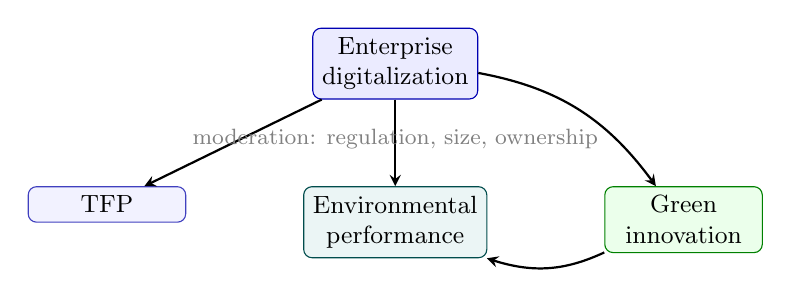
\begin{tikzpicture}[node distance=1.1cm and 1.6cm, every node/.style={font=\small}, box/.style={draw, rounded corners=3pt, minimum width=2cm, align=center}, arr/.style={->, >=stealth, thick}]
    \node[box, draw=blue!70!black, fill=blue!8] (X) {Enterprise\\digitalization};
    \node[box, below left=of X, draw=blue!50!gray, fill=blue!5] (TFP) {TFP};
    \node[box, below=of X, draw=teal!60!black, fill=teal!8] (Env) {Environmental\\performance};
    \node[box, below right=of X, draw=green!50!black, fill=green!8] (M) {Green\\innovation};
    \draw[arr] (X) -- (TFP);
    \draw[arr] (X) -- (Env);
    \draw[arr] (X) to[bend left=22] (M);
    \draw[arr] (M) to[bend left=22] (Env);
    \node[above=0.35cm of Env, font=\footnotesize, text=gray] {moderation: regulation, size, ownership};
  \end{tikzpicture}
  \caption{Conceptual framework (for reference only). Direct links: digitalization $\to$ TFP and digitalization $\to$ environmental performance. Mediation: digitalization $\to$ green innovation $\to$ environmental performance. Moderation: regulation strength and firm characteristics. The paper does not estimate or test these links; the figure illustrates the target structure and the measurement pitfalls when constructs are replaced by proxies.}
  \label{fig:model}
\end{figure}

% Sample construction flowchart (referenced in Methods)
\begin{figure}[t!]
  \centering
  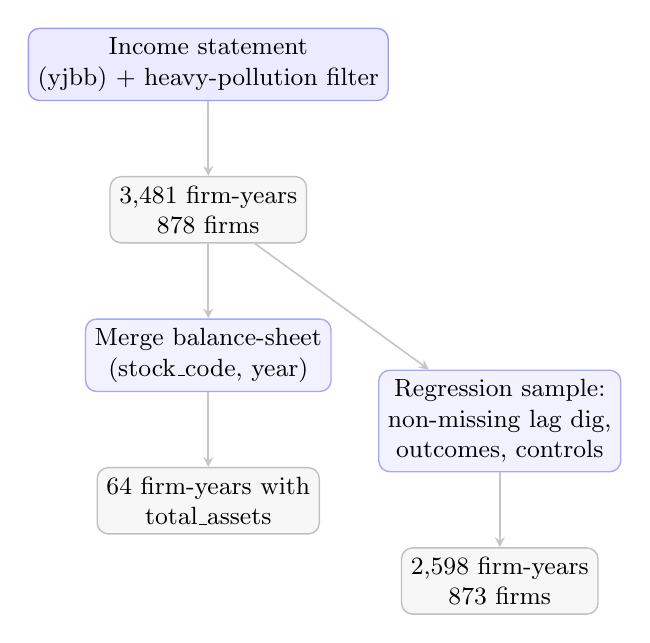
\begin{tikzpicture}[
    node distance=0.95cm and 1.5cm,
    every node/.style={font=\small},
    box/.style={draw=gray!50, rounded corners=4pt, minimum width=2.4cm, align=center, fill=white, line width=0.5pt},
    boxStart/.style={box, fill=blue!8, draw=blue!40},
    boxCount/.style={box, fill=gray!6},
    boxProcess/.style={box, fill=blue!5, draw=blue!35},
    arr/.style={->, >=stealth, draw=gray!45, line width=0.6pt}
  ]
    \node[boxStart] (A) {Income statement\\(yjbb) + heavy-pollution filter};
    \node[boxCount, below=of A] (B) {3,481 firm-years\\878 firms};
    \node[boxProcess, below=of B] (C) {Merge balance-sheet\\(stock\_code, year)};
    \node[boxCount, below=of C] (D) {64 firm-years with\\total\_assets};
    \node[boxProcess, below right=1.6cm and 0.9cm of B] (E) {Regression sample:\\non-missing lag dig,\\outcomes, controls};
    \node[boxCount, below=of E] (F) {2,598 firm-years\\873 firms};
    \draw[arr] (A) -- (B);
    \draw[arr] (B) -- (C);
    \draw[arr] (C) -- (D);
    \draw[arr] (B) -- (E);
    \draw[arr] (E) -- (F);
  \end{tikzpicture}
  \caption{Sample construction flowchart. Left column: merge path leading to 64 observations with total assets. Right branch: regression sample (size = ln(revenue)) used in Table~2.}
  \label{fig:sample-flow}
\end{figure}

% Figure 2: Descriptive time trend -- line plot (data from figure2_by_year.csv)
\pgfplotsset{
  fig2style/.style={
    width=6cm,
    height=5.5cm,
    xmin=2018.5, xmax=2022.5,
    xtick={2019,2020,2021,2022},
    xticklabel style={/pgf/number format/1000 sep={}},
    grid=both,
    major grid style={draw=gray!40, line width=0.4pt},
    minor grid style={draw=gray!20, line width=0.2pt},
    minor tick num=1,
    xlabel style={font=\small},
    ylabel style={font=\small},
    tick label style={font=\small},
    legend pos=south west,
    legend style={font=\small, draw=gray!60, fill=white, fill opacity=0.95, rounded corners=2pt, cells={anchor=west}, at={(axis description cs:0.02,0.05)}, anchor=south west},
    legend cell align=left,
  }
}
\begin{figure}[t!]
  \centering
  \resizebox{\textwidth}{!}{%
  \noindent
  \begin{minipage}[t]{6.2cm}
    \centering
    \begin{tikzpicture}
      \begin{axis}[fig2style,
        xlabel={Year},
        ylabel={Mean revenue (100M yuan)},
        ymin=0, ymax=100]
        \addplot[blue!80!black, mark=*, mark size=2.5pt, thick, smooth] coordinates {(2019,60.83) (2020,63.55) (2021,78.96) (2022,85.80)};
        \addlegendentry{Revenue (mean)}
      \end{axis}
    \end{tikzpicture}
  \end{minipage}%
  \hspace{0.4cm}%
  \begin{minipage}[t]{6.2cm}
    \centering
    \begin{tikzpicture}
      \begin{axis}[fig2style,
        xlabel={Year},
        ylabel={Mean ROE (\%)},
        ymin=0, ymax=12,
        legend pos=south east,
        legend style={font=\small, draw=gray!60, fill=white, fill opacity=0.95, rounded corners=2pt, cells={anchor=west}, at={(axis description cs:0.98,0.05)}, anchor=south east}]
        \addplot[teal!70!black, mark=square*, mark size=2pt, thick, smooth] coordinates {(2019,2.17) (2020,9.81) (2021,10.29) (2022,6.88)};
        \addlegendentry{ROE (mean)}
      \end{axis}
    \end{tikzpicture}
  \end{minipage}%
  }
  \caption{Descriptive trends: mean revenue (100 million yuan) and mean ROE (\%) by year (heavy-pollution firms, 2019--2022). Left: revenue; right: ROE.}
  \label{fig:descriptive}
\end{figure}

% =============================================================================
% TABLES (main text: descriptives + one proxy illustration only)
% =============================================================================

% Table 1: Full descriptive statistics (N, Mean, SD, Min, Max) -- from data/processed/table1_descriptives_full.csv
\begin{table}[t!]
  \centering
  \caption{Descriptive statistics and sample structure (heavy-pollution firms, 2019--2022).}
  \label{tab:descriptives}
  \small
  \begin{tabularx}{\textwidth}{@{}>{\raggedright\arraybackslash}X r r r r r@{}}
    \toprule
    Variable & $N$ & Mean & SD & Min & Max \\
    \midrule
    \multicolumn{6}{l}{\textit{Panel A: Sample structure}} \\
    Firm-year observations & 3,481 & -- & -- & -- & -- \\
    Unique firms & 878 & -- & -- & -- & -- \\
    Years & 2019--2022 & -- & -- & -- & -- \\
    Regression sample (non-missing lag dig, outcome) & 2,598 & -- & -- & -- & -- \\
    \midrule
    \multicolumn{6}{l}{\textit{Panel B: Main variables}} \\
    Revenue (100 million yuan) & 3,481 & 72.33 & 215.39 & 0.00 & 3,445.33 \\
    Total assets (100 million yuan) & 64 & 281.07 & 721.86 & 5.69 & 3,774.75 \\
    ROE (\%) & 3,467 & 9.40 & 16.57 & $-$74.94 & 54.02 \\
    Size (ln assets) & 64 & 22.17 & 1.79 & 20.16 & 26.66 \\
    Gross margin (\%) & 3,474 & 30.82 & 18.62 & $-$2.10 & 89.00 \\
    \bottomrule
  \end{tabularx}
  \vspace{0.5em}
  \parbox{\textwidth}{\raggedright\footnotesize\textit{Note.} $N$ = non-missing count per variable. Revenue and ROE from yjbb (AKShare). Total assets and size (ln assets) from balance-sheet merge by firm and year; only 64 firm-years match, so regressions use size = ln(revenue). Regression sample (Table~2): 2,598 firm-years (873 firms) after requiring non-missing lagged digitalization and outcome proxies.}
\end{table}

% Table 2: Proxy illustration (TFP and env.\ performance) -- from scripts/run_regressions.py
\begin{table}[t!]
  \centering
  \caption{Illustration: proxy-based regression. Outcome columns (1)--(2) = TFP proxy (ROE); (3)--(4) = environmental performance proxy (revenue growth). Regressor = lagged digitalization proxy (industry-year revenue rank). Not a test of the conceptual framework.}
  \label{tab:regression}
  \small
  \begin{tabularx}{\textwidth}{@{}>{\raggedright\arraybackslash}X c c c c@{}}
    \toprule
    & (1) TFP & (2) TFP & (3) Env. perf. & (4) Env. perf. \\
    \midrule
    Digitalization (lagged) & & $-$35.91 & & $-$3.00 \\
    & & (4.31) & & (0.06) \\
    Size (ln revenue) & Yes & Yes & Yes & Yes \\
    \midrule
    Firm fixed effects & Yes & Yes & Yes & Yes \\
    Year fixed effects & Yes & Yes & Yes & Yes \\
    \midrule
    Observations & 2,598 & 2,598 & 2,598 & 2,598 \\
    Unique firms & 873 & 873 & 873 & 873 \\
    $R^2$ & 0.031 & 0.056 & 0.224 & 0.580 \\
    \bottomrule
  \end{tabularx}
  \vspace{0.5em}
  \parbox{\textwidth}{\raggedright\footnotesize\textit{Note.} Columns (1)--(2): outcome = TFP proxy (ROE). Columns (3)--(4): outcome = environmental performance proxy (revenue growth). All columns: regressor $X_{i,t-1}$ = industry-year revenue rank (lagged). Control vector $\mathbf{Z}_{it}$: size = ln(revenue); firm and year fixed effects. Standard errors in parentheses; SEs are cluster-robust at firm level where applicable. 873 firms, 2,598 observations.}
\end{table}

% Table: Controlled experiment (validation + regression)
\begin{table}[htbp]
  \centering
  \caption{Controlled experiment: validation and regression.}
  \label{tab:synthetic-validation}
  \small
  \begin{tabularx}{\textwidth}{@{}Xcc@{}}
    \toprule
    & Value & Note \\
    \midrule
    \multicolumn{3}{l}{\textit{Panel A: Validation (Phase 3)}} \\
    Env.\ performance proxy (revenue growth): mean & 0.001 & \\
    Env.\ performance proxy: SD & 0.100 & \\
    Digitalization proxy (lagged rank): mean & 0.505 & \\
    Digitalization proxy: SD & 0.289 & \\
    Corr(true digitalization, revenue) & $-$0.008 & DGP: $\perp$ revenue \\
    \midrule
    \multicolumn{3}{l}{\textit{Panel B: Regression (env.\ proxy $\sim$ lag dig + FE)}} \\
    Coefficient (lagged digitalization) & $-$0.32 & \\
    SE & 0.038 & \\
    $t$-statistic & $-$8.42 & \\
    $N$ & 1,500 & 500 firms $\times$ 3 years \\
    \bottomrule
  \end{tabularx}
  \medskip
  \parbox{\textwidth}{\raggedright\footnotesize\textit{Note.} Panel: 500 firms, 4 years; true digitalization by design uncorrelated with revenue (seed 42). Validation confirms DGP; regression shows significant association from same-source structure only.}
\end{table}

% =============================================================================
% DISCUSSION (compressed for methodological note)
% =============================================================================

\section{Discussion}
\label{sec:discussion}

The value of this paper is methodological. We ask why revenue-based proxies mislead and how widespread the problem is. Our focus is not to estimate the causal effect but to show how proxy substitution alters identification. The \emph{literature audit} (Section~\ref{sec:related}) finds that 83\% (83 of 100) of audited firm-level studies use at least one revenue-related or accounting-based proxy; the issue is prevalent. Journal-tier classification is reported in \ref{app:audit-protocol}. We then show that regressions using revenue rank, ROE, and revenue growth study \emph{revenue dynamics}, not digitalization; same-source bias and construct mismatch make the coefficients uninterpretable for the double-dividend question. The controlled experiment (Section~\ref{sec:synthetic-experiment}, Table~\ref{tab:synthetic-validation}) confirms that significant associations can arise from measurement structure alone when true digitalization is by design uncorrelated with revenue. A reviewer might object that we only demonstrate revenue-based proxy $\to$ revenue-based outcome, which is mechanically correlated. Our point is that many studies in the literature use exactly this structure (revenue rank or similar for digitalization, revenue growth or ROE for outcomes). The controlled experiment shows that even when true digitalization is uncorrelated with revenue, this structure yields significant coefficients; hence results in such designs cannot distinguish a true digitalization effect from same-source structure. We do not claim that all proxy-based designs use this structure, but that the prevalent pattern we document does. We acknowledge that our illustration uses revenue-based outcomes; a demonstration using a non-revenue outcome (e.g., emission or GTFP where data are available) would further strengthen the critique; we encourage such work. Data and code will be deposited in a public repository upon acceptance. We document target vs.\ implemented design, sample flowchart, and merge diagnostics to support a \emph{blueprint} for valid inference: text-based digitalization, LP/OP TFP, emission or GTFP measures, green patents, and regional regulation. Section~\ref{sec:formal-diagnostic} adds a \emph{methodological} component: Proposition~1 formalizes same-source proxy bias; Corollary~1 shows that under monotone same-source proxies the coefficient sign is systematic (rationalizing the negative coefficients in our tables); Theorem~2 shows that the $t$-statistic can diverge with sample size, so false positives become more convincing in larger samples; Corollary~2 states that partial controls (e.g., size or fixed effects) do not eliminate the bias when residual source variation remains. The three-step diagnostic and practical checklist give applied researchers a concrete procedure; our controlled experiment implements the third step.

\textbf{Why significance is not reassurance.} A common empirical intuition is that large samples and robust standard errors provide reassurance. Our formal results show the opposite in same-source settings: if the population projection induced by proxy structure is nonzero (as in Corollary~1), standard asymptotics make the coefficient more, not less, convincingly significant (Theorem~2). In such cases, significance reflects persistence of the source structure rather than evidence on the target causal relationship.

\textbf{Contribution in context.} We provide \emph{formal results} (Proposition~1, Corollary~1, Theorem~2, Corollary~2) and a \emph{usable diagnostic} (three-step procedure plus practical checklist), in addition to the first structured audit of proxy use in this literature, a transparent illustration and controlled experiment, and a blueprint for valid inference. We do not propose a new estimator or identification strategy; the diagnostic allows researchers to assess whether their proxy-based estimates are likely driven by same-source structure. This combination (formal characterization of identification failure, directional bias, and spurious significance, plus diagnostic and demonstration) supports better empirical practice and meets the bar for a method-oriented contribution.

Limitations: the implemented variables do not measure the target constructs; we do not test the double dividend. Total assets match only 64 firm-years (Table~\ref{tab:merge-diagnostics}, Figure~\ref{fig:sample-flow}); we verified the merge and report it for transparency; commercial integrated data (e.g., CSMAR, WIND) could provide larger asset coverage. The IV specification uses a weak instrument (\ref{app:iv}). The sample is Chinese listed firms in heavily polluting industries. The audit covers 100 studies; \ref{app:audit-protocol} reports the protocol and journal-tier classification. The controlled experiment uses a minimal DGP; alternative specifications (e.g., AR(1), industry heterogeneity) could be explored. Some cited works are from 2025--2026 (early view or in press); we cite as of our search date. A valid test would require direct measures and quasi-experimental variation; this note's contribution is to clarify measurement failure and to point to that path.

% =============================================================================
% CONCLUSION
% Best practice: restate purpose, summarize contributions, implications,
% limitations/future work, closing takeaway.
% =============================================================================

\section{Conclusion}
\label{sec:conclusion}

This paper asked why revenue-based proxies mislead research on enterprise digitalization, environmental performance, and productivity, and how widespread that measurement problem is. We did not test whether digitalization improves both TFP and environmental performance (the double dividend). We showed that when researchers use revenue rank for digitalization, ROE for TFP, and revenue growth for environmental performance, regressions capture revenue dynamics rather than the target constructs, and we provided evidence that this pattern is common in the literature.

We documented \emph{prevalence} through a structured audit of 100 firm-level studies: 83\% use at least one revenue-related or accounting-based proxy. We \emph{formalized} same-source proxy bias (Proposition~1), showed that monotone same-source proxies imply a systematic sign and non-vanishing bias (Corollary~1), and that the $t$-statistic can diverge as the sample grows (Theorem~2). We gave a three-step diagnostic and a practical checklist so that applied researchers can assess whether their estimates are likely driven by proxy structure. We \emph{demonstrated} measurement failure with a transparent proxy-based illustration on Chinese A-share firms in heavily polluting industries and with a controlled experiment in which true digitalization is by design uncorrelated with revenue yet the proxy regression remains significant. We also provided a \emph{blueprint} for valid inference: text-based digitalization measures, production-function TFP, emission or GTFP for environmental performance, and strong instruments where needed.

The implications are twofold. For applied researchers, the diagnostic (Section~\ref{sec:formal-diagnostic}) offers a concrete way to check for same-source risk before interpreting proxy regressions as causal. For the literature on digitalization and environment or productivity, our audit suggests that many existing results may conflate revenue or accounting variation with the theoretical constructs; replication and re-estimation with direct measures would clarify the evidence. Limitations are discussed in Section~\ref{sec:discussion} (sample, data merge, audit scope, minimal DGP). Future work could extend the audit to more studies and journal tiers, replicate the diagnostic on published specifications, and test the double dividend with direct measures and quasi-experimental variation.

We do not claim substantive findings on the double dividend. We claim a clear methodological contribution: the measurement problem is common, identification of the target relationship requires direct measures and a design that avoids same-source proxy structure, and the paper supplies a formal characterization, a diagnostic, and a path for rigorous testing in a policy-relevant domain.


\appendix
\renewcommand{\thesection}{Appendix~\Alph{section}}
\section{Additional regression tables and figures}
\label{app:extra-tables}

For transparency we report mediation, moderation, robustness, and the coefficient and moderation plots. These do not support inference; they illustrate proxy behavior only.

% Table 3: Mediation
\begin{table}[htbp]
  \centering
  \caption{Mediation equation with proxy mediator (ROE improvement). Not a test of green-innovation mediation.}
  \label{tab:mediation}
  \small
  \begin{tabularx}{\textwidth}{@{}>{\raggedright\arraybackslash}X c c c@{}}
    \toprule
    & (1) Env. perf. & (2) Green innov. & (3) Env. perf. \\
    \midrule
    Digitalization (lagged) & $-$3.00 & $-$20.36 & $-$2.98 \\
    & (0.06) & (4.60) & (0.06) \\
    Green innovation & & & 0.001 \\
    & & & (0.0003) \\
    Size (ln revenue), Firm FE, Year FE & Yes & Yes & Yes \\
    \midrule
    Observations & 2,598 & 2,598 & 2,598 \\
    Indirect effect & -- & -- & $-$0.023 \\
    \bottomrule
  \end{tabularx}
\end{table}

% Table 4: Moderation
\begin{table}[htbp]
  \centering
  \caption{Moderation by year, gross margin, and size. Year is a time trend, not environmental regulation.}
  \label{tab:moderation}
  \small
  \begin{tabularx}{\textwidth}{@{}>{\raggedright\arraybackslash}X c c c@{}}
    \toprule
    & (1) Year & (2) Margin & (3) Size \\
    \midrule
    Digitalization (lagged) & $-$3.03 & $-$3.00 & $-$2.91 \\
    & (0.06) & (0.06) & (0.06) \\
    Digitalization $\times$ Moderator & 0.044 & 0.003 & 0.389 \\
    & (0.012) & (0.001) & (0.026) \\
    \midrule
    Observations & 2,598 & 2,598 & 2,598 \\
    \bottomrule
  \end{tabularx}
\end{table}

% Table 5: Robustness
\begin{table}[htbp]
  \centering
  \caption{Robustness: alternative outcome and alternative digitalization proxy.}
  \label{tab:robustness}
  \small
  \begin{tabularx}{\textwidth}{@{}>{\raggedright\arraybackslash}X c c@{}}
    \toprule
    & (1) Alt. outcome (ROE) & (2) Alt. dig. (ln revenue pctl) \\
    \midrule
    Digitalization (lagged) & $-$35.91 & $-$3.18 \\
    & (4.31) & (0.06) \\
    \midrule
    Observations & 2,598 & 1,725 \\
    \bottomrule
  \end{tabularx}
\end{table}

% Figure 3: Coefficient plot (appendix)
\begin{figure}[htbp]
  \centering
  \resizebox{\textwidth}{!}{%
  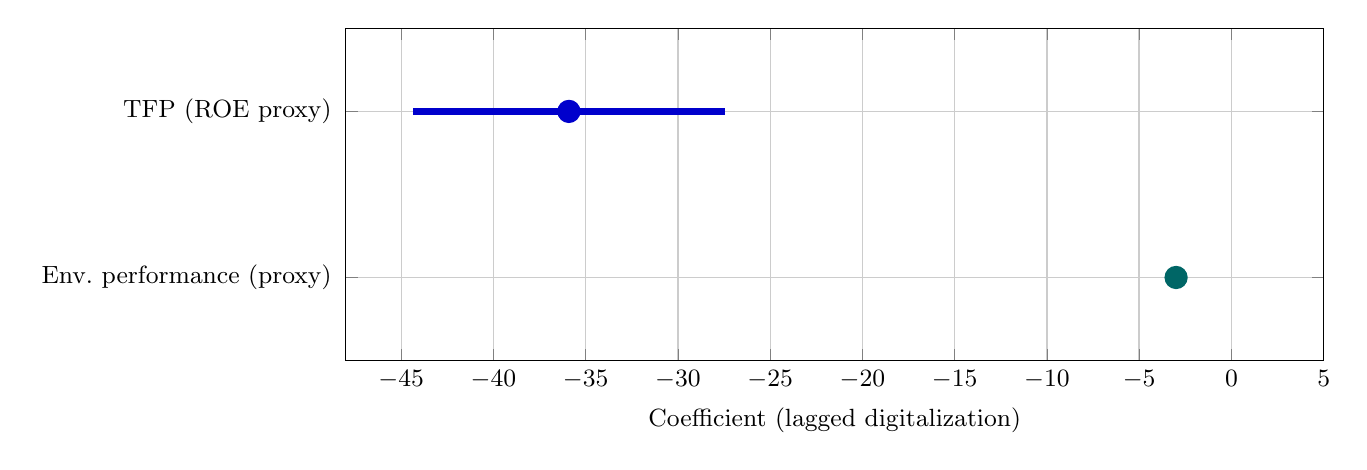
\begin{tikzpicture}
    \begin{axis}[width=14cm, height=5.8cm, xlabel={Coefficient (lagged digitalization)}, yticklabels={Env.\ performance (proxy), TFP (ROE proxy)}, ytick={1,2}, ymin=0.5, ymax=2.5, xmin=-48, xmax=5, grid=both, major grid style={draw=gray!40, line width=0.5pt}, xlabel style={font=\small}, tick label style={font=\small}, yticklabel style={align=right, inner sep=0.5em}]
      \addplot[teal!80!black, no markers, line width=2.5pt] coordinates {(-3.12,1) (-2.88,1)};
      \addplot[teal!80!black, only marks, mark=*, mark size=4pt] coordinates {(-3.00,1)};
      \addplot[blue!80!black, no markers, line width=2.5pt] coordinates {(-44.36,2) (-27.46,2)};
      \addplot[blue!80!black, only marks, mark=*, mark size=4pt] coordinates {(-35.91,2)};
    \end{axis}
  \end{tikzpicture}%
  }
  \caption{Coefficient plot: main effects from Table~\ref{tab:regression} (columns 2 and 4).}
  \label{fig:coefficients}
\end{figure}

% Figure 4: Moderation plot (appendix)
\begin{figure}[t!]
  \centering
  \resizebox{\textwidth}{!}{%
  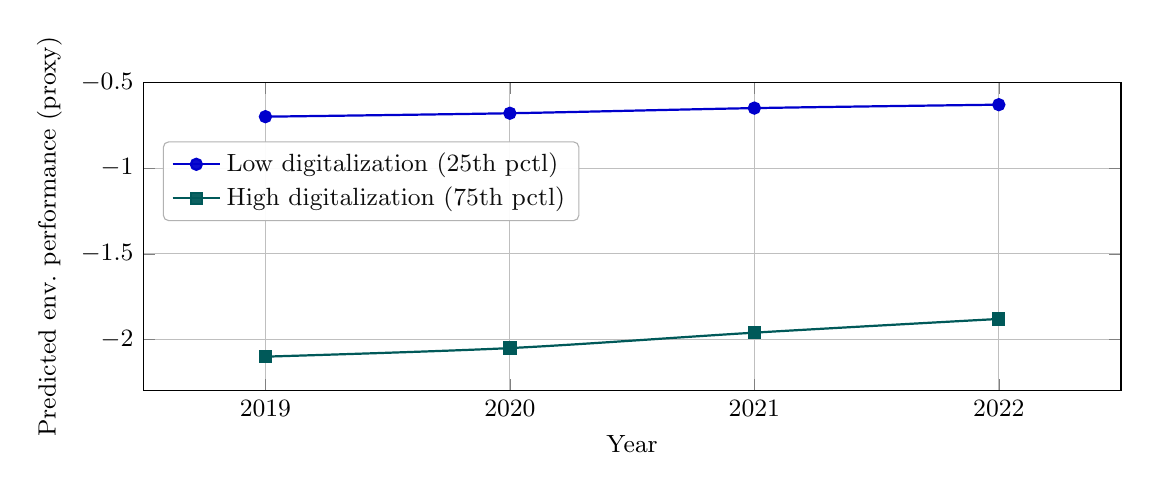
\begin{tikzpicture}
    \begin{axis}[width=14cm, height=5.5cm, xlabel={Year}, ylabel={Predicted env.\ performance (proxy)}, xtick={2019,2020,2021,2022}, xticklabel style={/pgf/number format/1000 sep={}}, xmin=2018.5, xmax=2022.5, ymin=-2.3, ymax=-0.5, grid=both, legend style={at={(axis description cs:0.02,0.55)}, anchor=south west, font=\small, draw=gray!60, fill=white, fill opacity=0.95, rounded corners=2pt, cells={anchor=west}}, legend cell align=left, font=\small]
      \addplot[blue!80!black, mark=*, thick, smooth] coordinates {(2019,-0.70) (2020,-0.68) (2021,-0.65) (2022,-0.63)};
      \addlegendentry{Low digitalization (25th pctl)}
      \addplot[teal!70!black, mark=square*, thick, smooth] coordinates {(2019,-2.10) (2020,-2.05) (2021,-1.96) (2022,-1.88)};
      \addlegendentry{High digitalization (75th pctl)}
    \end{axis}
  \end{tikzpicture}%
  }
  \caption{Moderation by year (from Table~\ref{tab:moderation}, column 1). Year is a time trend, not regulation.}
  \label{fig:interaction}
\end{figure}

\section{Instrumental-variable specification (weak instrument)}
\label{app:iv}

We estimated a 2SLS specification using the two-year lag of the digitalization proxy as the instrument. The first-stage $F$-statistic is 2.02, well below the conventional threshold of 10; the IV estimates are therefore \emph{not reliable} for inference and are relegated to this appendix. We do not use them to support any causal claim.

\begin{table}[t!]
  \centering
  \caption{IV specification (for transparency only; weak instrument).}
  \label{tab:app-iv}
  \small
  \begin{tabularx}{\textwidth}{@{}Xcc@{}}
    \toprule
    & First stage & Second stage \\
    \midrule
    Instrument (2-year lag dig.) & 0.032 & \\
    & (0.023) & \\
    Fitted digitalization (lagged) & & $-$6.91 \\
    & & (2.92) \\
    \midrule
    First-stage $F$ & 2.02 & \\
    Observations & 1,725 & 1,725 \\
    \bottomrule
  \end{tabularx}
  \medskip
  \parbox{\textwidth}{\raggedright\footnotesize\textit{Note.} Standard errors in parentheses. Instrument is two-year lag of digitalization proxy. $F = 2.02$ indicates weak instrument; second-stage estimates are not interpretable for causal inference.}
\end{table}

\section{Protocol for extended literature audit (100--300 studies)}
\label{app:audit-protocol}

This appendix documents the audit protocol and reporting. The main text reports an audit of 100 studies (83\% proxy use). Below we specify the screening steps and journal-tier classification used.

\textbf{Step 1 -- Identification.} Search Web of Science, Scopus, and CNKI (2018--2024). Query: (``enterprise digitalization'' OR ``digital transformation'') AND (``environmental performance'' OR ``green TFP'' OR ``TFP'' OR ``productivity''). Record initial hit counts per database. Export to a single list; deduplicate by title and DOI. Record $N$ unique records.

\textbf{Step 2 -- Screening.} Title and abstract screening: retain only records that mention at least two of (digitalization, TFP/productivity, environmental performance) in a firm-level or comparable empirical context. Record exclusions by reason (irrelevant topic, no firm-level, review/theory only, other). Record $M$ records passing to full text.

\textbf{Step 3 -- Eligibility.} Full-text assessment: retain only English or Chinese; empirical firm-level (or comparable); at least two of the three constructs present; sufficient measurement detail to classify each construct. Record exclusions by reason (no measurement detail, not firm-level, duplicate, other). Record $K$ records included.

\textbf{Step 4 -- Classification.} For each of the $K$ studies, code: (a) digitalization measure (direct: text-based/validated index; proxy: revenue rank, composite embedding revenue, etc.); (b) TFP/productivity measure (direct: LP/OP or equivalent; proxy: ROE, revenue-based productivity, etc.); (c) environmental measure (direct: emission intensity, GTFP; proxy: ESG when used in place of emission, revenue growth, etc.). Classify journal tier: top field (e.g., JEEM, JEM, Research Policy, JBE, SMJ); mid-tier (field journals with impact factor above median); policy/other.

\textbf{Step 5 -- Reporting.} Report PRISMA flowchart: identification $\to$ screening $\to$ eligibility $\to$ included ($K$). Report prevalence (share of $K$ using at least one revenue-related or accounting-based proxy) overall and by journal tier. A table of the form [Study | Journal | Tier | Digitalization | TFP | Environmental | Any proxy?] can be placed in an online appendix. The full list of the 100 audited studies (with classification) is included in the replication package and available from the authors upon request.

\bibliography{references}

\end{document}
